\label{kap:hudba}
\mathquote{Hudba je skryté cvičení v aritmetice, při kterém duše neví, že počítá.}{Gottfried Wilhelm Leibniz}

V kapitole~\ref{kap:priroda} jsme viděli, že tón je kmitání vzduchu, že kvinta je poměr frekvencí $3:2$ a že dvanáct kvint se nikdy úplně nepotká se sedmi oktávami. V této kapitole půjdeme hlouběji. Proč zní některé dvojice tónů dobře a jiné ne? Proč má oktáva právě dvanáct půltónů a ne deset? Proč je mollový akord zrcadlovým obrazem durového? A jak souvisí Eukleidův algoritmus s africkými a kubánskými rytmy? Hudební teorie je z velké části matematika, jen se o tom v hudebce moc nemluví.

\section{Struna a řada alikvotních tónů}

Napnutá struna délky $L$, upevněná na obou koncích, může kmitat jen tak, aby na koncích zůstala v klidu. Vejde se na ni půl vlny, celá vlna, jeden a půl vlny, a tak dál. Jde o stojaté vlnění z kapitoly~\ref{kap:diferencialni}.

\begin{center}
  \begin{tikzpicture}[x=5cm, y=0.55cm]
    \foreach \n in {1,2,3,4} {
      \begin{scope}[yshift={-(\n-1)*1.5cm}]
        \draw[gray] (0,0) -- (1,0);
        \draw[thick, colorofwisdom, domain=0:1, samples=80] plot (\x, {sin(180*\n*\x)});
        \draw[colorofwisdom!40, domain=0:1, samples=80] plot (\x, {-sin(180*\n*\x)});
        \foreach \k in {0,...,\n} \fill ({\k/\n},0) circle (1.4pt);
        \node[anchor=west, font=\small] at (1.05,0) {$f_{\n} = \n f_1$};
      \end{scope}
    }
  \end{tikzpicture}
\end{center}

Vlnová délka $n$-tého módu je $\frac{2L}{n}$, a tedy jeho frekvence je $n$-násobkem základní frekvence $f_1$. Struna přitom kmitá všemi módy najednou. Slyšíme tón o frekvenci $f_1$, ale `obarvený' vyššími \textbf{alikvotními tóny} (harmonickými) $2f_1$, $3f_1$, $4f_1$, \dots Totéž platí pro vzduchový sloupec ve flétně nebo trubce. Na strunu ale můžeme `zahrát' i jednotlivé alikvóty: když se struny kytary v polovině jen lehce dotknete, utlumíte módy s lichým $n$ a zazní flažolet o oktávu výš.

Základní frekvenci struny popisují \textbf{Mersennovy zákony} (1636):
\begin{equation*}
  f_1 = \frac{1}{2L}\sqrt{\frac{T}{\mu}},
\end{equation*}
kde $T$ je napětí a $\mu$ hmotnost jednoho metru struny. Poloviční délka dává dvojnásobnou frekvenci (to je pražec v polovině hmatníku). Čtyřnásobné napětí také dvojnásobnou. A proto jsou basové struny tlusté a ovinuté drátem: velké $\mu$ snižuje tón, aniž by struna musela být metry dlouhá.

\subsection*{Alikvoty jako stupnice}

Vynesme si alikvotní tóny tónu $C$ na osu, na které stejná vzdálenost znamená stejný \textit{poměr} frekvencí (tedy na logaritmickou osu z kapitoly~\ref{kap:exponencialni}). Přesně takhle totiž výšku tónu vnímá ucho.

\begin{center}
  \begin{tikzpicture}[x=3cm]
    \draw[->] (0,0) -- (4.15,0) node[right, font=\scriptsize] {$\log_2\frac{f}{f_1}$};
    \foreach \o in {0,1,2,3,4} \draw[gray] (\o,0.1) -- (\o,-0.1) node[below, font=\scriptsize] {\o};
    \foreach \n/\l in {1/C, 2/c, 3/g, 4/c^1, 5/e^1, 6/g^1, 7/, 8/c^2, 9/d^2, 10/e^2, 11/, 12/g^2, 13/, 14/, 15/h^2, 16/c^3} {
      \pgfmathsetmacro{\p}{ln(\n)/ln(2)}
      \draw[very thick, colorofwisdom] (\p,0.15) -- (\p,0.75);
      \node[font=\tiny, above] at (\p,0.75) {\n};
      \node[font=\tiny, below] at (\p,-0.35) {$\l$};
    }
    \node[font=\scriptsize, anchor=west] at (0,1.4) {čísla alikvotů nad čarou, jména tónů pod osou (oktávy jsou stejně dlouhé)};
  \end{tikzpicture}
\end{center}

V první oktávě je jen jeden alikvot, ve druhé přibude kvinta, ve třetí tercie a kvinta, a čím výš, tím hustěji. Uprostřed se objevují přesně ty intervaly, na kterých stojí evropská hudba. Oktáva $2:1$, kvinta $3:2$, kvarta $4:3$, velká tercie $5:4$, malá tercie $6:5$. Durový akord $c^1$, $e^1$, $g^1$ je doslova poskládaný z alikvotů číslo $4$, $5$ a $6$. Proto se mu říká `přirozený'. Alikvoty $7$, $11$, $13$ a $14$ jsme nepojmenovali. Do běžné stupnice nepasují, a právě z nich mají svůj typický zvuk třeba alpské rohy.

\section{Intervaly: násobení, ne sčítání}

Interval je \textit{poměr} frekvencí. Zahrát kvintu a pak ještě kvartu znamená vynásobit frekvenci $\frac{3}{2}\cdot\frac{4}{3} = 2$, tedy dohromady oktávu. Ucho ale intervaly vnímá, jako by se \textit{sčítaly}. Mezi násobením a sčítáním je most, který už známe: logaritmus.

\begin{definitionbox}
  Velikost intervalu s poměrem frekvencí $r = \frac{f_2}{f_1}$ v \textbf{centech} je
  \begin{equation*}
    c(r) = 1200\log_2 r.
  \end{equation*}
  Oktáva má $1200$ centů a rovnoměrně temperovaný půltón přesně $100$. Platí $c(r_1r_2) = c(r_1) + c(r_2)$, takže skládání intervalů je obyčejné sčítání centů.
\end{definitionbox}

\begin{center}
  \begin{tabular}{|l|c|c|c|c|}
    \hline
    interval & čistý poměr & centy (čistě) & centy (temperovaně) & rozdíl\\
    \hline
    malá tercie & $6:5$ & $315{,}6$ & $300$ & $-15{,}6$\\
    velká tercie & $5:4$ & $386{,}3$ & $400$ & $+13{,}7$\\
    kvarta & $4:3$ & $498{,}0$ & $500$ & $+2{,}0$\\
    kvinta & $3:2$ & $702{,}0$ & $700$ & $-2{,}0$\\
    malá sexta & $8:5$ & $813{,}7$ & $800$ & $-13{,}7$\\
    velká sexta & $5:3$ & $884{,}4$ & $900$ & $+15{,}6$\\
    oktáva & $2:1$ & $1200$ & $1200$ & $0$\\
    \hline
  \end{tabular}
\end{center}

Rozdíl jednoho centu je na hranici toho, co trénované ucho rozezná. Kvinty a kvarty klavíru jsou tedy skoro čisté. Tercie jsou o celou sedminu půltónu vedle. Pěvecké sbory a smyčcová kvarteta, které nemají pevné ladění, proto tercie intuitivně `opravují' k čistým poměrům.

\section{Proč zní konsonance dobře}

Proč zrovna jednoduché poměry? Jedna odpověď je vidět přímo na průběhu vlny. Sečtěme dvě sinusovky s poměrem frekvencí $3:2$ a dvě s poměrem $\sqrt{2}$ (rovnoměrně temperovaný tritón, `ďábel v hudbě'):

\begin{center}
  \begin{tikzpicture}[x=0.42cm, y=0.5cm]
    \draw[gray] (0,0) -- (25.2,0);
    \draw[thick, colorofwisdom, domain=0:25.13, samples=300] plot (\x, {sin(deg(2*\x))+sin(deg(3*\x))});
    \foreach \k in {0,1,2,3,4} \draw[dashed, gray] ({6.2832*\k},-2.1) -- ({6.2832*\k},2.1);
    \node[anchor=west, font=\scriptsize] at (25.6,0) {kvinta $3:2$};
    \begin{scope}[yshift=-2.6cm]
      \draw[gray] (0,0) -- (25.2,0);
      \draw[thick, gray!70!black, domain=0:25.13, samples=300] plot (\x, {sin(deg(2*\x))+sin(deg(2.8284*\x))});
      \node[anchor=west, font=\scriptsize] at (25.6,0) {tritón $\sqrt{2}:1$};
    \end{scope}
  \end{tikzpicture}
\end{center}

Kvinta dává periodický průběh, který se opakuje po každé druhé periodě nižšího tónu (čárkované čáry), protože $\mathrm{nsn}(2, 3)$ je malé číslo. U poměru $\sqrt{2}$ se vzor nikdy přesně neopakuje, protože $\sqrt{2}$ je iracionální. Druhá odpověď je v alikvotech (kapitola~\ref{kap:priroda}): u jednoduchého poměru mají oba tóny mnoho společných alikvotů a zbylé jsou od sebe daleko. U složitého poměru leží alikvoty obou tónů těsně vedle sebe a vytvářejí rychlé zázněje, které ucho vnímá jako drsnost. Moderní psychoakustika (Plomp a Levelt, 1965) tuto drsnost měří a z alikvotů dokáže předpovědět, které intervaly budou znít libě.

\section{Spirála kvint a dvanáct tónů}

Pythagorejci stavěli stupnici z kvint. Začneme na $c$, jdeme o kvintu výš na $g$, pak na $d$, $a$, $e$, \dots, a kdykoli vyletíme z oktávy, vydělíme frekvenci dvěma. Na kružnici, na které jeden oběh je jedna oktáva, je kvinta otočení o $360^\circ\cdot\log_2\frac{3}{2}\approx 210{,}6^\circ$. Kdyby se dvanáct kvint potkalo se sedmi oktávami, dvanáctý krok by nás vrátil přesně na start. Nevrátí, a tak místo kruhu kreslíme spirálu:

\begin{center}
  \begin{tikzpicture}[scale=1.15]
    \draw[gray!50] (0,0) circle (1.2);
    \foreach \n/\a/\l in {0/0/c, 1/210.59/g, 2/61.17/d, 3/271.76/a, 4/122.35/e, 5/332.93/h, 6/183.52/fis, 7/34.11/cis, 8/244.69/gis, 9/95.28/dis, 10/305.87/ais, 11/156.45/eis, 12/7.04/his} {
      \pgfmathsetmacro{\r}{1.2+0.11*\n}
      \coordinate (P\n) at ({90-\a}:\r);
      \fill[colorofwisdom] (P\n) circle (1.6pt);
      \node[font=\scriptsize] at ({90-\a}:{\r+0.3}) {$\l$};
    }
    \foreach \n [evaluate=\n as \m using int(\n+1)] in {0,...,11} \draw[colorofwisdom!50, ->, shorten >=2pt, shorten <=2pt] (P\n) -- (P\m);
    \draw[thick, dashed] (0,0) -- (90:2.9);
    \draw[thick, dashed] (0,0) -- (82.96:2.9);
    \node[font=\scriptsize, align=left, anchor=west] at (0.4,3.05) {Pythagorejské koma\\$\approx 23{,}5$ centu};
  \end{tikzpicture}
\end{center}

Tón $his$ po dvanácti kvintách je o $23{,}46$ centu (asi čtvrtinu půltónu) výš než $c$. Na obrázku je to malý úhel mezi dvěma čárkovanými přímkami. Tomu se říká \textbf{Pythagorejské koma} a celé dějiny ladění jsou dějinami toho, kam ho schovat.

\begin{note}
  Proč se spirála nikdy neuzavře, ať uděláme kvint kolik chceme? Kdyby ${\left(\frac{3}{2}\right)}^a = 2^b$ pro přirozená $a$, $b$, pak $3^a = 2^{a+b}$. Vlevo je ale liché číslo a vpravo sudé, což podle základní věty aritmetiky z kapitoly~\ref{kap:teorie-cisel} nejde. Ekvivalentně: číslo $\log_2\frac{3}{2}$ je iracionální.
\end{note}

\section{Odbočka --- Proč má oktáva právě dvanáct tónů}

Když se kruh čistých kvint přesně uzavřít nedá, můžeme se ptát, na kolik stejných dílů rozdělit oktávu, aby se v nich čistá kvinta schovala co nejlépe. Při rozdělení na $n$ dílů hledáme celé číslo $k$, pro které je $\frac{k}{n}$ co nejblíž
\begin{equation*}
  \log_2\frac{3}{2} = 0{,}584\,962\,5\ldots
\end{equation*}
Jde o úlohu přiblížit iracionální číslo zlomkem se jmenovatelem co nejmenším. Přesně tu řeší \textbf{řetězové zlomky} z odbočky v kapitole~\ref{kap:priroda}:
\begin{equation*}
  \log_2\frac{3}{2} = \cfrac{1}{1 + \cfrac{1}{1 + \cfrac{1}{2 + \cfrac{1}{2 + \cfrac{1}{3 + \cdots}}}}}
\end{equation*}
Useknutím dostaneme nejlepší přiblížení (sblížené zlomky)
\begin{equation*}
  \frac{1}{2},\quad\frac{3}{5},\quad\frac{7}{12},\quad\frac{24}{41},\quad\frac{31}{53},\quad\dots
\end{equation*}
Zlomek $\frac{7}{12}$ znamená: kvinta je $7$ půltónů z $12$. Zlomek $\frac{3}{5}$ odpovídá pětitónové (pentatonické) stupnici, kterou najdeme v lidové hudbě po celém světě. Graf ukazuje, jak daleko je nejlepší kvinta při rozdělení oktávy na $n$ dílů od čisté kvinty:

\begin{center}
  \begin{tikzpicture}[x=0.215cm, y=1cm]
    \draw[->] (4,0) -- (55,0) node[right, font=\scriptsize] {$n$};
    \draw[->] (4,0) -- (4,2.5) node[above, font=\scriptsize] {chyba kvinty (centy)};
    \foreach \c in {10,20,30,40,50} \draw[gray!40] (4,{\c*0.045}) -- (54,{\c*0.045}) node[right, font=\tiny, gray] {\c};
    \foreach \n/\h in {6/2.25,7/0.73,8/2.16,9/1.59,10/0.81,11/2.13,13/1.64,14/0.73,15/0.81,16/1.21,17/0.18,18/1.41,19/0.32,20/0.81,21/0.73,22/0.32,23/1.07,24/0.09,25/0.81,26/0.43,27/0.41,28/0.73,29/0.07,30/0.81,31/0.23,32/0.47,33/0.50,34/0.18,35/0.73,36/0.09,37/0.52,38/0.32,39/0.26,40/0.54,42/0.55,43/0.19,44/0.32,45/0.39,46/0.11,47/0.57,48/0.09,49/0.37,50/0.27,51/0.18,52/0.43} {
      \fill[gray!55] ({\n-0.35},0) rectangle ({\n+0.35},\h);
    }
    \foreach \n/\h in {5/0.81,12/0.09,41/0.02,53/0.00} {
      \fill[colorofwisdom] ({\n-0.35},0) rectangle ({\n+0.35},{max(\h,0.02)});
      \node[font=\scriptsize, colorofwisdom, above] at (\n,{\h+0.05}) {\n};
    }
  \end{tikzpicture}
\end{center}

Dvanáctka je nejmenší počet dílů, při kterém je chyba kvinty menší než dva centy, tedy pod hranicí slyšitelnosti. Menší počty buď kvintu minou o hodně, nebo (jako $n = 7$) vedou ke stupnici, ve které jsou intervaly příliš hrubé. Dalšími `rekordmany' jsou $41$ a $53$. Rozdělení na $53$ dílů navrhl už v 1. století př.\,n.\,l. čínský teoretik Ťing Fang a kolem $53$ dílů oktávy je postavena i teorie tradiční turecké hudby. Dvanáct tónů tedy není výmysl skladatelů ani kulturní náhoda. Je to nejlepší kompromis mezi počtem kláves a čistotou kvint.

\subsection*{Syntonické koma}

Kvinty nejsou jediný problém. Čtyři čisté kvinty nahoru a dvě oktávy dolů by měly dát velkou tercii. Dají ale
\begin{equation*}
  {\left(\frac{3}{2}\right)}^4\cdot\frac{1}{4} = \frac{81}{64}\qquad\text{místo}\qquad\frac{5}{4} = \frac{80}{64}.
\end{equation*}
Poměr $\frac{81}{80}$ (asi $21{,}5$ centu) je \textbf{syntonické koma}. Čisté kvinty a čisté tercie tedy nejdou mít zároveň. Renesanční \textit{středotónové ladění} proto kvinty trochu zúžilo, aby vycházely čisté tercie. V oblíbených tóninách to znělo krásně, ve vzdálených tóninách ale vznikla tzv. vlčí kvinta, tak falešná, že `vyla'. Rovnoměrné ladění, které se prosadilo v 18. a 19. století, rozpustilo všechna komata rovnoměrně do všech intervalů. Žádná tónina není dokonalá, ale všechny jsou stejně použitelné.

\section{Hudba v modulární aritmetice}

V hudbě se tóny lišící se o oktávu považují za `stejné' ($c$, $c^1$ i $c^2$ jsou všechny $c$). Pojmenujeme-li půltóny čísly
\begin{equation*}
  c = 0,\ cis = 1,\ d = 2,\ \dots,\ h = 11,
\end{equation*}
počítáme s nimi \textbf{modulo 12}, přesně jako s hodinami v kapitole~\ref{kap:teorie-cisel}. Tóny tvoří grupu $\mathbb{Z}_{12}$.

\begin{center}
  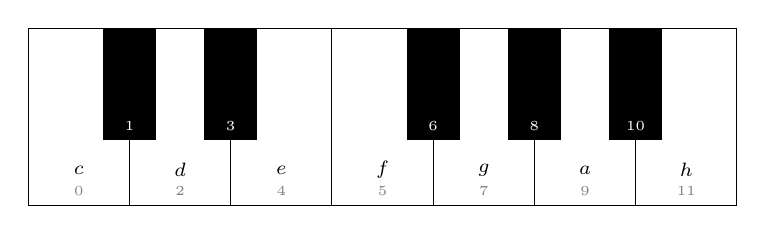
\begin{tikzpicture}[x=0.75cm, y=0.75cm]
    \foreach \x/\l/\k in {0/c/0, 1/d/2, 2/e/4, 3/f/5, 4/g/7, 5/a/9, 6/h/11} {
      \draw ({\x*1.7143},0) rectangle ({(\x+1)*1.7143},3);
      \node[font=\scriptsize] at ({(\x+0.5)*1.7143},0.6) {$\l$};
      \node[font=\tiny, gray] at ({(\x+0.5)*1.7143},0.25) {\k};
    }
    \foreach \b/\k in {1.7143/1, 3.4286/3, 6.8571/6, 8.5714/8, 10.2857/10} {
      \fill ({\b-0.45},1.1) rectangle ({\b+0.45},3);
      \node[font=\tiny, white] at (\b,1.35) {\k};
    }
  \end{tikzpicture}
\end{center}

\begin{definitionbox}
  \textbf{Transpozice} o $n$ půltónů je zobrazení $T_n(x) = x + n \bmod 12$. \textbf{Inverze} (zrcadlení) je $I(x) = -x \bmod 12$. Na hodinovém ciferníku tónů je transpozice otočení a inverze překlopení. Dohromady generují grupu symetrií pravidelného dvanáctiúhelníku se $24$ prvky.
\end{definitionbox}

\begin{center}
  \begin{tikzpicture}[scale=1.25]
    \foreach \k/\l in {0/c, 1/cis, 2/d, 3/dis, 4/e, 5/f, 6/fis, 7/g, 8/gis, 9/a, 10/ais, 11/h} {
      \coordinate (T\k) at ({90-30*\k}:1.5);
      \fill (T\k) circle (1.3pt);
      \node[font=\scriptsize] at ({90-30*\k}:1.82) {$\l$};
    }
    \draw[gray!40] (0,0) circle (1.5);
    \fill[colorofwisdom!35, opacity=0.8] (T0) -- (T4) -- (T7) -- cycle;
    \draw[thick, colorofwisdom] (T0) -- (T4) -- (T7) -- cycle;
    \draw[thick, dashed] (T0) -- (T3) -- (T7) -- cycle;
    \draw[gray, dash dot] ({90-30*3.5}:2.1) -- ({90-30*9.5}:2.1);
    \node[font=\scriptsize, colorofwisdom, align=center] at (2.9,0.6) {C dur\\$\{0, 4, 7\}$};
    \node[font=\scriptsize, align=center] at (2.9,-0.6) {c moll\\$\{0, 3, 7\}$};
  \end{tikzpicture}
\end{center}

Durový akord $\{0, 4, 7\}$ se skládá z velké tercie ($4$ půltóny) a malé tercie ($3$). Mollový akord $\{0, 3, 7\}$ má tytéž intervaly v obráceném pořadí. Na ciferníku je to vidět okamžitě: c moll je zrcadlový obraz C dur podle osy, která leží mezi $dis$ a $e$ (čerchovaně). Zrcadlení $x\mapsto 7 - x$ totiž posílá $0\mapsto 7$, $4\mapsto 3$, $7\mapsto 0$. Všech $12$ durových a $12$ mollových akordů je tedy jediný trojúhelník v $24$ polohách, otočený a překlopený všemi symetriemi dvanáctiúhelníku.

Některé akordy jsou souměrnější než jiné. Zvětšený kvintakord $\{0, 4, 8\}$ je rovnostranný trojúhelník: transpozice o $4$ ho nezmění, a proto existují jen $4$ různé zvětšené akordy. Zmenšený septakord $\{0, 3, 6, 9\}$ je čtverec a existují jen $3$. Právě kvůli této souměrnosti zní tyto akordy `nejistě' a skladatelé je rádi používají k nečekaným modulacím: akord se dá rozvést mnoha směry, protože patří do mnoha tónin zároveň.

\section{Rytmus a Eukleidův algoritmus}

Matematika není jen ve výšce tónů, ale i v čase. Hrají-li dva hudebníci zároveň tři a dva stejně dlouhé údery na takt, potkají se jejich údery jen na začátku taktu a takt se přirozeně dělí na $\mathrm{nsn}(3, 2) = 6$ dílků. Tomu se říká \textbf{polyrytmus} $3:2$.

\begin{center}
  \begin{tikzpicture}[x=1.2cm, y=0.7cm]
    \foreach \i in {0,...,6} \draw[gray!50] (\i,-0.4) -- (\i,1.4);
    \foreach \i in {0,2,4} \fill[colorofwisdom] ({\i+0.5},1) circle (4pt);
    \foreach \i in {0,3} \fill ({\i+0.5},0) circle (4pt);
    \node[anchor=east, font=\scriptsize] at (-0.1,1) {3 údery};
    \node[anchor=east, font=\scriptsize] at (-0.1,0) {2 údery};
    \foreach \i in {1,...,6} \node[font=\tiny, gray] at ({\i-0.5},-0.7) {\i};
  \end{tikzpicture}
\end{center}

Zajímavější úloha: jak rozmístit $k$ úderů mezi $n$ pulzů co nejrovnoměrněji? Matematik Godfried Toussaint si v roce 2005 všiml, že algoritmus, který tuto úlohu řeší (a který byl původně vymyšlen pro časování neutronových zdrojů v urychlovačích částic), je ve skutečnosti Eukleidův algoritmus z kapitoly~\ref{kap:teorie-cisel}. A že rytmy, které vytváří, se objevují v tradiční hudbě po celém světě. Říká se jim \textbf{eukleidovské rytmy} $E(k, n)$.

\begin{center}
  \begin{tikzpicture}[scale=1]
    \foreach \cx/\hits/\name in {0/{0,3,6}/{$E(3, 8)$: tresillo}, 4.5/{0,2,3,5,6}/{$E(5, 8)$: cinquillo}} {
      \begin{scope}[xshift=\cx cm]
        \draw[gray!50] (0,0) circle (1.2);
        \foreach \k in {0,...,7} \draw[gray] ({90-45*\k}:1.2) circle (3pt);
        \foreach \k in \hits \fill[colorofwisdom] ({90-45*\k}:1.2) circle (4pt);
        \node[font=\scriptsize] at (0,-1.75) {\name};
      \end{scope}
    }
  \end{tikzpicture}
\end{center}

Tři údery mezi osm pulzů, $x\,.\,.\,x\,.\,.\,x\,.$, je \textbf{tresillo}, rytmický základ kubánské hudby, reggaetonu i spousty současného popu. Pět úderů mezi osm, $x\,.\,x\,x\,.\,x\,x\,.$, je kubánské \textbf{cinquillo}. Eukleidův algoritmus pro $\mathrm{NSD}(8, 3)$ dělí `$8 = 2\cdot 3 + 2$' a přesně tato dělení určují, jak velké mezery mezi údery vzniknou: dvě mezery délky $3$ a jedna délky $2$.

\section{Barva zvuku a Fourier}

Proč zní $a^1$ na flétně jinak než na houslích, když mají stejnou frekvenci $440$ Hz? Protože mají jiné \textbf{spektrum}, tedy jiné zastoupení alikvotů. Každý periodický tón lze podle kapitoly~\ref{kap:rady} rozložit na Fourierovu řadu
\begin{equation*}
  p(t) = \sum_{n=1}^{\infty}a_n\sin(2\pi nf_1t + \varphi_n),
\end{equation*}
a právě čísla $a_n$ slyšíme jako barvu zvuku. Flétna má skoro čistý sinusový tón s několika slabými alikvoty. Klarinet má díky válcové trubici zesílené liché alikvoty a jeho tón připomíná obdélníkovou vlnu. Housle mají bohaté spektrum, protože smyčec strunu opakovaně chytá a pouští a struna kmitá jako pilovitá vlna, ve které jsou zastoupeny všechny alikvoty s amplitudou zhruba $\frac{1}{n}$.

Syntezátory to dělají obráceně. \textbf{Aditivní syntéza} skládá zvuk ze sinusovek. \textbf{Subtraktivní syntéza} začne u pilovité nebo obdélníkové vlny s bohatým spektrem a filtrem z ní ubírá vysoké alikvoty. Autotune a rozpoznávání skladeb v mobilu zase zvuk nejprve rozloží na frekvence pomocí \textit{rychlé Fourierovy transformace}, algoritmu, který spočítá spektrum $n$ vzorků přibližně za $n\log n$ kroků místo $n^2$.

\begin{problem}
  \begin{enumerate}[label=(\alph*)]
    \item Kolik centů má interval s poměrem $\frac{9}{8}$ (Pythagorejský celý tón)? Porovnejte s temperovaným celým tónem.
    \item Struna dlouhá $65$ cm zní tónem $110$ Hz. Kde musí být pražec, aby zněla kvinta výš?
    \item Ukažte, že dvanáct temperovaných kvint dá přesně sedm oktáv.
    \item Najděte v $\mathbb{Z}_{12}$ obraz durového akordu $\{0, 4, 7\}$ při inverzi $I(x) = -x$. O jaký akord jde?
    \item Kolik různých zmenšených septakordů $\{x, x + 3, x + 6, x + 9\}$ existuje?
  \end{enumerate}
\end{problem}

\begin{solution}
  \begin{enumerate}[label=(\alph*)]
    \item $1200\log_2\frac{9}{8}\approx 203{,}9$ centu, temperovaný celý tón má $200$.
    \item Frekvence je nepřímo úměrná délce, takže znějící část musí mít délku $\frac{2}{3}\cdot 65\approx 43{,}3$ cm. Pražec je tedy asi $21{,}7$ cm od nultého pražce u hlavy kytary, ve třetině struny.
    \item ${\left(2^{7/12}\right)}^{12} = 2^7$. Temperovaná kvinta je tím pádem o přesně $\frac{1}{12}$ Pythagorejského komatu užší než čistá.
    \item $\{0, 8, 5\} = \{f, gis, c\}$, tedy f moll ($gis = as$).
    \item Tři. Akord se nezmění transpozicí o $3$, takže z $12$ transpozic jsou různé jen $\frac{12}{4} = 3$.
  \end{enumerate}
\end{solution}

\section{Příběh --- Kníže, který vraždil a skládal}

Carlo Gesualdo, kníže z Venosy, byl synovcem kardinála a jedním z nejbohatších šlechticů neapolského království. V říjnu 1590 v Neapoli přistihl svou ženu Marii d'Avalos s jejím milencem, vévodou z Andrie, a oba i s pomocí sluhů zavraždil. Těla nechal vystavit před palácem. Potrestán nebyl: podle tehdejších představ šlechtic hájil svou čest.

Gesualdo se pak stáhl na svůj hrad, znovu se oženil a skládal. Jeho pozdní madrigaly, třeba \textit{Moro, lasso, al mio duolo} (`Umírám, běda, ve své bolesti'), jsou plné chromatických postupů a akordů ze vzdálených tónin, které po sobě jdou tak nečekaně, že jim hudební teoretici dodnes zkoumají logiku. Zněly o tři staletí moderněji, než bylo v jeho době zvykem, a takové harmonie se naplno prosadily až s rovnoměrným laděním, kde mají všechny tóniny stejnou cenu. Igor Stravinskij Gesualda obdivoval a k 400. výročí jeho narození napsal skladbu \textit{Monumentum pro Gesualdo}.

Podle dobových zpráv trpěl Gesualdo na konci života těžkými depresemi a nechával se denně bičovat svými sluhy. Zemřel v roce 1613 na svém hradě v Gesualdu, jen několik týdnů po svém jediném synovi z prvního manželství.

\section{Shrnutí a otázky}

\begin{problem}
  Odpovězte vlastními slovy:
  \begin{enumerate}
    \item Proč struna nekmitá jen jednou frekvencí? Co jsou alikvotní tóny?
    \item Co říkají Mersennovy zákony? Proč jsou basové struny tlusté?
    \item Proč se intervaly měří v centech a proč je to logaritmus?
    \item Proč zní jednoduché poměry frekvencí libě? Uveďte dvě vysvětlení.
    \item Co je Pythagorejské a syntonické koma? Proč se spirála kvint nikdy neuzavře?
    \item Proč má oktáva dvanáct půltónů? Jak s tím souvisí řetězové zlomky?
    \item Jak lze tóny popsat jako $\mathbb{Z}_{12}$? Proč je mollový akord zrcadlovým obrazem durového?
    \item Co jsou eukleidovské rytmy?
    \item Co určuje barvu zvuku a jak s ní souvisí Fourierova řada?
  \end{enumerate}
\end{problem}
